\documentclass[final_report.tex]{subfiles}

\begin{document}

\section{DPDK}
%https://embedded.communities.intel.com/thread/6828
%http://dpdk.org/ml/archives/dev/2013-June/000237.html
\label{sec:dpdk}
This section will go into much more detail about the Data Plane Development Kit (DPDK), focussing on the basic concepts used by the fast packet processing framework for use within custom applications. DPDK does have a number of more advanced features which can be exploited but aren't discussed in this report. \todo{ref manual}

\subsection{Environment Abstraction Layer (EAL)}
The EAL abstracts the specific environment from the user and provides a constant interface in order for applications to be ported to other environments without problems. The EAL compilation may change depending on the architecture (32-bit or 64-bit), operating system, compilers in use or network interface cards. This is done via the creation of a set of libraries that are environment specific and are responsible for the low-level operations gaining access to hardware and memory resources.

On the start-up of an application, the EAL is responsible for finding PCI information about devices and addresses via the igb\_uio kernel module, performing physical memory allocation using huge pages (section \ref{subsec:hugepages}) and starting user-level threads for the logical cores (section \ref{subsec:logical_cores}) (lcores) of the application. 

\subsection{Logical Cores}
\label{subsec:logical_cores}
%http://www.tomshardware.co.uk/forum/306079-28-what-core-thread
%https://computing.llnl.gov/tutorials/pthreads/
%https://en.wikipedia.org/wiki/Native_POSIX_Thread_Library
%http://stackoverflow.com/questions/1888160/distinguish-java-threads-and-os-threads
%http://wimhesselink.nl/pub/whh241b.pdf
Also know as lcores within DPDK, logical cores shouldn't be confused with processor cores. Lcores are threads which allow different applications functions to be run within different threads. This can allow different lcores to control different ports and queues while processing packets as well.

Within DPDK lcores are implemented with POSIX threads (on linux) and make use of processor affinity (CPU pinning). This allows lcores to be only run on certain processing cores which reduces context switching and cache memory swapping and therefore increasing overall perforamance. However, this only works of the number of lcores is equal or less than the number of available processing cores so the number of lcores which are allowed to be initiated are limited. This feature can also exploit modern processors which allow for hyper-threaded cores but the performance increase isn't as guarenteed as it is with non-hyper-threaded cores.

\subsection{Huge Pages}
%https://www.kernel.org/doc/Documentation/vm/hugetlbpage.txt
%https://access.redhat.com/documentation/en-US/Red_Hat_Enterprise_Linux/6/html/Performance_Tuning_Guide/s-memory-transhuge.html
\label{subsec:hugepages}
Huge pages are a way of increasing performance when dealing with large amounts of memory. Normally, memory is managed in 4096 byte (4KB) blocks known as pages, which are listed within the CPU memory management unit (MMU). However, if a system uses a large amount of memory, increasing the number of standard pages is expensive on the CPU as the MMU can only handle thousands of pages and not millions.

The solution is to increase the page size from 4KB to 2MB or 1GB (if supported) which keeps the number of pages references small in the MMU but increases the overall memory for the system. Huge pages should be assigned at boot time for better overall management, but can be manual assigned on initial boot up if required.

DPDK makes uses of huge pages simply for increased performance due to the large amount of packets in memory. This is even the case if the system memory size is relatively small and the application isn't processing an extreme number of packets.

\subsection{Ring Buffer}
A ring buffer is used by DPDK to manage transmit and receive queues for each network port on the system. This fixed sized first-in-first-out queue allows multiple objects to be enqueued and dequeued from the ring at the same time from any number of consumers or producers. A major disadvantage of this is that once the ring is full (more of a concern in receive queues), it allows no more objects can be added to the ring, resulting in dropped packets or packet caches. It is therefore imperative that applications can processes packets at the required rate.

\begin{figure}[H]
	\centering
	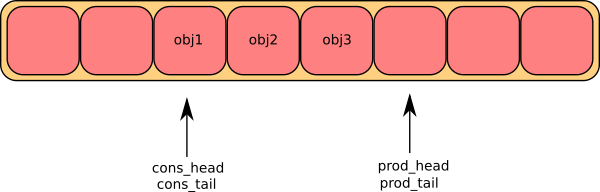
\includegraphics[width=\textwidth]{img/ring.png}
	\caption{Ring Buffer}
	\label{fig:ring}
\end{figure}
\todo{cite this}

\subsection{Memory Usage}
DPDK tries to regulate memory usage in order to be more efficient and therefore handles its own memory management. However, it does allow application to allocate memory blocks for specific port queues and for data sharing between lcores. The major memory techniques used are described below.

\todo[inline]{should code use dpdk malloc?}

\subsubsection{Allocation}
Since DPDK make use of huge pages, it provides its own memory allocation (malloc) library to allow memory blocks of any size, which also improves the portability of applications. However, even the DPDK malloc library is slow compared to pool memory access due to synchronisation constraints. Generally this library should only be used at initialisation time but does support NUMA for specific socket memory access and memory alignment.

\subsubsection{Pools}
Memory pools allow for fixed size allocation of memory which uses a ring to store fixed sized objects. These a almost guarenteed to be used for message buffer storage for receive and transmit queues for ports. They are initialised with a number of paremeters to increas performance such as cache sizes and NUMA socked identification as well as a name identify.

Pools offer increased performance over the standard memory allocation since the object padding is optimised so each object starts on a different memory channel and rank. Furthermore, a per core cache can be enabled at initialisation. This offers performance advantages, as without caching per core locks are required for every pool access. Caches offer cores lock free access to data, while bulk requested can be carried out on the pool to reduce locking on the pool.

\subsubsection{Message Buffers}
Message Buffers (mbufs) are stored within a specified memory pool and are used to carry data between different processes within the application and are primarily used for carrying network packets through the application. Mbufs also contain metadata about the information it is carrying which includes the data length, message type and offsets for the start of the data. The headroom shown in figure \ref{fig:mbuf} shows empty bytes between the metadata and start of the data which allows the data to be memory aligned for quicket access. Mbufs can also be chained together to allow for longer data, more commonly jumbo packets.

\begin{figure}[H]
	\centering
	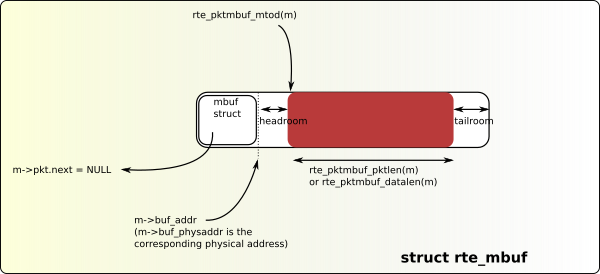
\includegraphics[width=\textwidth]{img/mbuf.png}
	\caption{Message Buffer}
	\label{fig:mbuf}
\end{figure}
\todo{cite this}

\subsubsection{NUMA}
DPDK can make use of non-uniform memory access (NUMA) if the system supports it. NUMA is a method for speeding up memory access when multiple processors are trying to access the same memory and therefore reduces the processors waiting time. Each processor will receive its own bank of memory which is faster to access as it doesn't have to wait. As applications become more extensive, processors may need to share memory, which is possible via moving the data between memory banks. This somewhat negates the need for NUMA, but NUMA can be very effective depending on the application. DPDK can make extensive use of NUMA as each logical core is generally responsible for its own queues, and since queues can't be shared between logical cores (although dedicated ring buffers can), data sharing is rare.

\begin{figure}[H]
	\centering
	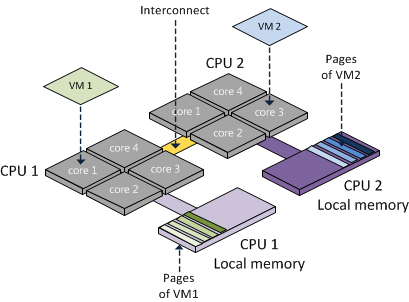
\includegraphics[width=\textwidth/2]{img/numa.png}
	\caption{NUMA}
	\label{fig:numa}
\end{figure}
\todo{cite this}

\subsection{Poll Mode Driver (PMD)}
A Poll Mode Driver (PMD) is a user space device which allows configuration of network interface cards/controllers and their associated queues. PMD's work without interrupts which allow for quicker recieving, processing and transmitting of packets and are therefore lock free. Generally anything which can be achieved by interrupts can also be achived via using rings and continuous polling of the rings. This means that 2 lcores running in parallel can't receive from the same queue on the same port. However, 2 parallel cores can receive from the same port on different queues.

There a number of consideration for application design depending on the hardware in use. Optimal performance can be achieved by carefully considering the hardware properties such as caches, bus speed and bandwidth along side the software design choices. For example, NIC's are more efficient at transmitting multiple packets in a burst rather than individually but consequently overalll throughput may be reduced.

\subsection{Models}
DPDK supports 2 methods for packet processing applications:

\paragraph*{Pipe-line}
This is an asychronous model where lcores a designated to perform certain tasks. Generally certain lcores will receive packets via the PMD api and simply pass those packets to other lcores via the use of a ring. These other lcores will then process the packets depending the requirements and then either forward the packets to the PMD for transmitting or pass them onto other lcore via a ring.

\paragraph*{Run-to-completion}
This is a synchronous model where each lcore will retrieve the packets, process them individually and then output them for transmission. Each lcore should be assigned its own receive and transmit queue on a given port in order to negate the need for locks. This report will focus on the run-to-completion model.

\end{document}